\documentclass{article}

\usepackage[T1]{fontenc}
\usepackage[utf8]{inputenc}
\usepackage[greek,english]{babel}
\usepackage[a4paper, margin=0.2in]{geometry}
\usepackage{CJKutf8}

\usepackage{tikz}
\usepackage{float}
\usetikzlibrary{arrows}

\begin{document}
\begin{CJK}{UTF8}{gbsn}

\title{hw2}
\author{刘本嵩 U201614531}

\maketitle

% \foreignlanguage{greek}{φΔδ} \begin{CJK}{UTF8}{gbsn}汉\end{CJK}

\section{Q3.8}
\Large
\smallskip

我们假设编译好的程序使得流水线依次执行下面几条计算指令: 
$ r1=A_1*B_1, r2=A_2*B_2, r3=A_3*B_3, r4=A_4*B_4, 
r5=r1+r2, r6=r3+r4, r7=r5+r6 $

然后画出时空图

\begin{figure}[H]
\centering
\includegraphics[scale=1]{hw2-img1.png}
\caption{时空图}
\end{figure}

注意到, 18个$\Delta t$输出了7个结果, 所以吞吐率

$$TP = \frac{7}{18\Delta t}$$

如果不用流水线, 一次乘法共$4\Delta t$, 加法$4\Delta t$, 共$7*4\Delta t = 28\Delta t$, 有加速比

$$S = \frac{28\Delta t}{18\Delta t} = 1.556$$

流水线的效率用面积比值求出,

$$E=\frac{4*7}{18*5}=0.311 = 31.111\%$$

\section{Q3.10}
\Large
\smallskip

(1) Forbidden list = ${1,3,6}$, Collision Vector = $100101$. So we have the state graph:

\begin{figure}[H]
\centering
    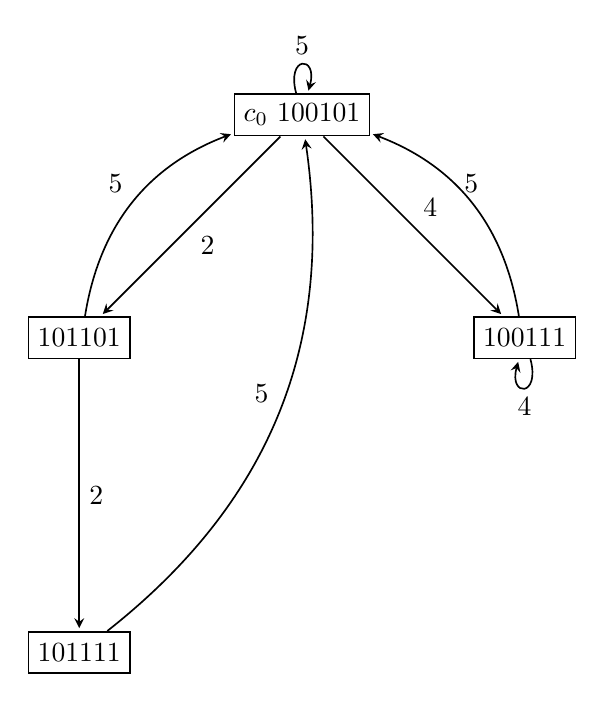
\begin{tikzpicture}[
            > = stealth, % arrow head style
            shorten > = 1pt, % don't touch arrow head to node
            auto,
            node distance = 4cm, % distance between nodes
            semithick, % line style
            state/.style = {shape=rectangle,draw,minimum size=1.5em}
        ]

        \node[state] (top)                      {$c_0$ 100101};
        \node[state] (l1)  [below left of=top]  {101101};
        \node[state] (l2)  [below of=l1]        {101111};
        \node[state] (r1)  [below right of=top] {100111};
        \path[->] (top) edge              node        {2} (l1);
        \path[->] (top) edge              node        {4} (r1);
        \path[->] (top) edge [loop above] node        {5} (top);
        \path[->] (l1)  edge [bend left]  node        {5} (top);
        \path[->] (l2)  edge [bend right] node        {5} (top);
        \path[->] (r1)  edge [bend right] node [above]{5} (top);
        \path[->] (l1)  edge              node        {2} (l2);
        \path[->] (r1)  edge [loop below] node        {4} (r1);
    \end{tikzpicture}
\caption{state graph}
\end{figure}

(2) 各种策略表

\begin{figure}[H]
\centering
 \begin{tabular}{||c|c||}
 \hline
     调度策略&平均延迟周期数 \\ [0.5ex]
 \hline\hline
     (2,5) & 3.5 \\
 \hline
     (2,2,5) & 3  \\
 \hline
     (5) & 5 \\
 \hline
     (4) & 4 \\
 \hline
     (4,5) & 4.5 \\ [1ex]
 \hline
\end{tabular}
\caption{strategy table}
\end{figure}

显然, 等间隔方案最小延迟为4, 不等间隔最小延迟为3. 等间隔最大吞吐率

$$TP=\frac{1}{4\Delta t}$$

不等间隔最大吞吐率

$$TP=\frac{1}{3\Delta t}$$

(3) 等间隔方案, 延迟为4, 共41个周期, 计算了10个输出. 吞吐率

$$TP=\frac{10}{41\Delta t}$$

$$SpeedUpRate=\frac{50\Delta t}{41\Delta t}=1.220$$

不等间隔方案, 延迟为3, 共32个周期, 计算了10个输出. 吞吐率

$$TP=\frac{10}{32\Delta t}$$

$$SpeedUpRate=\frac{50\Delta t}{32\Delta t}=1.563$$

\section{Q3.11}
\Large
\smallskip

(1) 没有其他重定向硬件, 流水线时空图如下

\begin{figure}[H]
\centering
\includegraphics[scale=0.6]{hw2-img2.png}
\caption{时空图}
\end{figure}

第i次循环的开始周期为$17i+1$, 总周期数$(98*17)+18=1684$.

(2) 有重定向硬件, 流水线时空图如下

\begin{figure}[H]
\centering
\includegraphics[scale=0.8]{hw2-img3.png}
\caption{时空图}
\end{figure}

第i次循环的开始周期为$10i+1$, 总周期数$(98*10)+11=991$.

(3) 使用延迟分支之后, 机器码顺序改为

\begin{verbatim}
LOOP: 
LW      R1, 0(R2)
DADDIU  R2,R2,#4 
DADDIU  R1,R1,#1 
DSUB    R4,R3,R2 
BNEZ    R4,LOOP 
SW      R1,-4(R2)
\end{verbatim}

\begin{figure}[H]
\centering
\includegraphics[scale=0.8]{hw2-img4.png}
\caption{时空图}
\end{figure}

第i次循环的开始周期为$6i+1$, 总周期数$(98*6)+10=598$.

\end{CJK}
\end{document}

